\documentclass[UTF8]{ctexart}

\usepackage{graphicx}

\title{算法分析与设计选做第二次作业}
\author{57119134 黄浩}
\date{\today}
\begin{document}
\maketitle

证明下述结论。

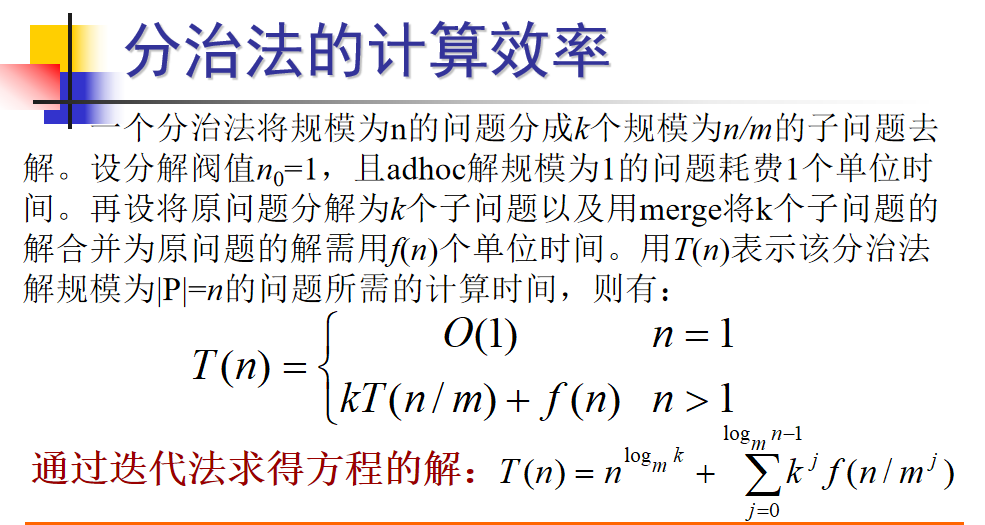
\includegraphics[width = 1\textwidth]{1.png}

证明:

\qquad 我们可以分析每一层的复杂度,再加上最后一层的复杂度从而得到总复杂度:

\qquad 第零层:$1$个节点,并开销 $f(n)$

\qquad 第一层: $k$个节点,并开销 $k\cdot f(n/m)$

\qquad 第二层:$k^2$个节点,并开销$k^2 \cdot f(n/m^2)$

\qquad 第三层:$k^3$个节点,并开销$k^3 \cdot f(n/m^3)$

\qquad $\cdots$

\qquad 第x层: $k^x$个节点,并开销$k^x \cdot f(n/m^x)$

\qquad $\cdots$

\qquad 由上我们也易知最后一层的叶子数为 $k^{log_mn} = n^{log_mk}$,所以最后一层的最简问题开销为$n^{log_mk}$。

\qquad 所以,我们将每一层的开销和最终最简问题的开销求和即是问题总开销:(注:最后一层由于已经是最简问题了,所以最后一层没有分解子问题的开销)

\qquad $T(n) = n^{log_mk} + \sum_{j = 0}^{log_mn - 1}k^j \cdot f(n/m^j)$

\qquad 得证。

另外:

\qquad 我们可以总结出一些直接得出递归式计算复杂度的方法:

\qquad 当$O(n^{log_mk}) < O(f(n))$时,$T(n) = O(f(n))$

\qquad 当$O(n^{log_mk}) = O(f(n))$时,$T(n) = O(n^{log_mk} \cdot log_mn)$

\qquad 当$O(n^{log_mk}) > O(f(n))$时,$T(n) = O(n^{log_mk})$

\end{document}